\documentclass[12pt,a4paper]{article}


\usepackage[in, plain]{fullpage}
\usepackage{array}
\usepackage{../../../pas-math}

%-------------------------------------------------------------------------------
%          -Packages nécessaires pour écrire en Français et en UTF8-
%-------------------------------------------------------------------------------
\usepackage[utf8]{inputenc}
\usepackage[frenchb]{babel}
\usepackage[T1]{fontenc}
\usepackage{lmodern}
\usepackage{textcomp}



%-------------------------------------------------------------------------------

%-------------------------------------------------------------------------------
%                          -Outils de mise en forme-
%-------------------------------------------------------------------------------
\usepackage{hyperref}
\hypersetup{pdfstartview=XYZ}
%\usepackage{enumerate}
\usepackage{graphicx}
\usepackage{multicol}
\usepackage{tabularx}
\usepackage{multirow}


\usepackage{anysize} %%pour pouvoir mettre les marges qu'on veut
%\marginsize{2.5cm}{2.5cm}{2.5cm}{2.5cm}

\usepackage{indentfirst} %%pour que les premier paragraphes soient aussi indentés
\usepackage{verbatim}
\usepackage{enumitem}
\usepackage[usenames,dvipsnames,svgnames,table]{xcolor}

\usepackage{variations}

%-------------------------------------------------------------------------------


%-------------------------------------------------------------------------------
%                  -Nécessaires pour écrire des mathématiques-
%-------------------------------------------------------------------------------
\usepackage{amsfonts}
\usepackage{amssymb}
\usepackage{amsmath}
\usepackage{amsthm}
\usepackage{tikz}
\usepackage{xlop}
%-------------------------------------------------------------------------------



%-------------------------------------------------------------------------------


%-------------------------------------------------------------------------------
%                    - Mise en forme avancée
%-------------------------------------------------------------------------------

\usepackage{ifthen}
\usepackage{ifmtarg}


\newcommand{\ifTrue}[2]{\ifthenelse{\equal{#1}{true}}{#2}{$\qquad \qquad$}}

%-------------------------------------------------------------------------------

%-------------------------------------------------------------------------------
%                     -Mise en forme d'exercices-
%-------------------------------------------------------------------------------
%\newtheoremstyle{exostyle}
%{\topsep}% espace avant
%{\topsep}% espace apres
%{}% Police utilisee par le style de thm
%{}% Indentation (vide = aucune, \parindent = indentation paragraphe)
%{\bfseries}% Police du titre de thm
%{.}% Signe de ponctuation apres le titre du thm
%{ }% Espace apres le titre du thm (\newline = linebreak)
%{\thmname{#1}\thmnumber{ #2}\thmnote{. \normalfont{\textit{#3}}}}% composants du titre du thm : \thmname = nom du thm, \thmnumber = numéro du thm, \thmnote = sous-titre du thm

%\theoremstyle{exostyle}
%\newtheorem{exercice}{Exercice}
%
%\newenvironment{questions}{
%\begin{enumerate}[\hspace{12pt}\bfseries\itshape a.]}{\end{enumerate}
%} %mettre un 1 à la place du a si on veut des numéros au lieu de lettres pour les questions 
%-------------------------------------------------------------------------------

%-------------------------------------------------------------------------------
%                    - Mise en forme de tableaux -
%-------------------------------------------------------------------------------

\renewcommand{\arraystretch}{1.7}

\setlength{\tabcolsep}{1.2cm}

%-------------------------------------------------------------------------------



%-------------------------------------------------------------------------------
%                    - Racourcis d'écriture -
%-------------------------------------------------------------------------------

% Angles orientés (couples de vecteurs)
\newcommand{\aopp}[2]{(\vec{#1}, \vec{#2})} %Les deuc vecteurs sont positifs
\newcommand{\aopn}[2]{(\vec{#1}, -\vec{#2})} %Le second vecteur est négatif
\newcommand{\aonp}[2]{(-\vec{#1}, \vec{#2})} %Le premier vecteur est négatif
\newcommand{\aonn}[2]{(-\vec{#1}, -\vec{#2})} %Les deux vecteurs sont négatifs

%Ensembles mathématiques
\newcommand{\naturels}{\mathbb{N}} %Nombres naturels
\newcommand{\relatifs}{\mathbb{Z}} %Nombres relatifs
\newcommand{\rationnels}{\mathbb{Q}} %Nombres rationnels
\newcommand{\reels}{\mathbb{R}} %Nombres réels
\newcommand{\complexes}{\mathbb{C}} %Nombres complexes


%Intégration des parenthèses aux cosinus
\newcommand{\cosP}[1]{\cos\left(#1\right)}
\newcommand{\sinP}[1]{\sin\left(#1\right)}


%Probas stats
\newcommand{\stat}{statistique}
\newcommand{\stats}{statistiques}
%-------------------------------------------------------------------------------

%-------------------------------------------------------------------------------
%                    - Mise en page -
%-------------------------------------------------------------------------------

\newcommand{\twoCol}[1]{\begin{multicols}{2}#1\end{multicols}}


\setenumerate[1]{font=\bfseries,label=\textit{\alph*})}
\setenumerate[2]{font=\bfseries,label=\arabic*)}


%-------------------------------------------------------------------------------
%                    - Elements cours -
%-------------------------------------------------------------------------------




\title{Correction des de la feuille 3 sur les angles}
\date{}


\graphicspath{{./img/}}
\begin{document}
	
\maketitle

\vspace*{-1cm}

\section*{Exercice 37}

\begin{center}
	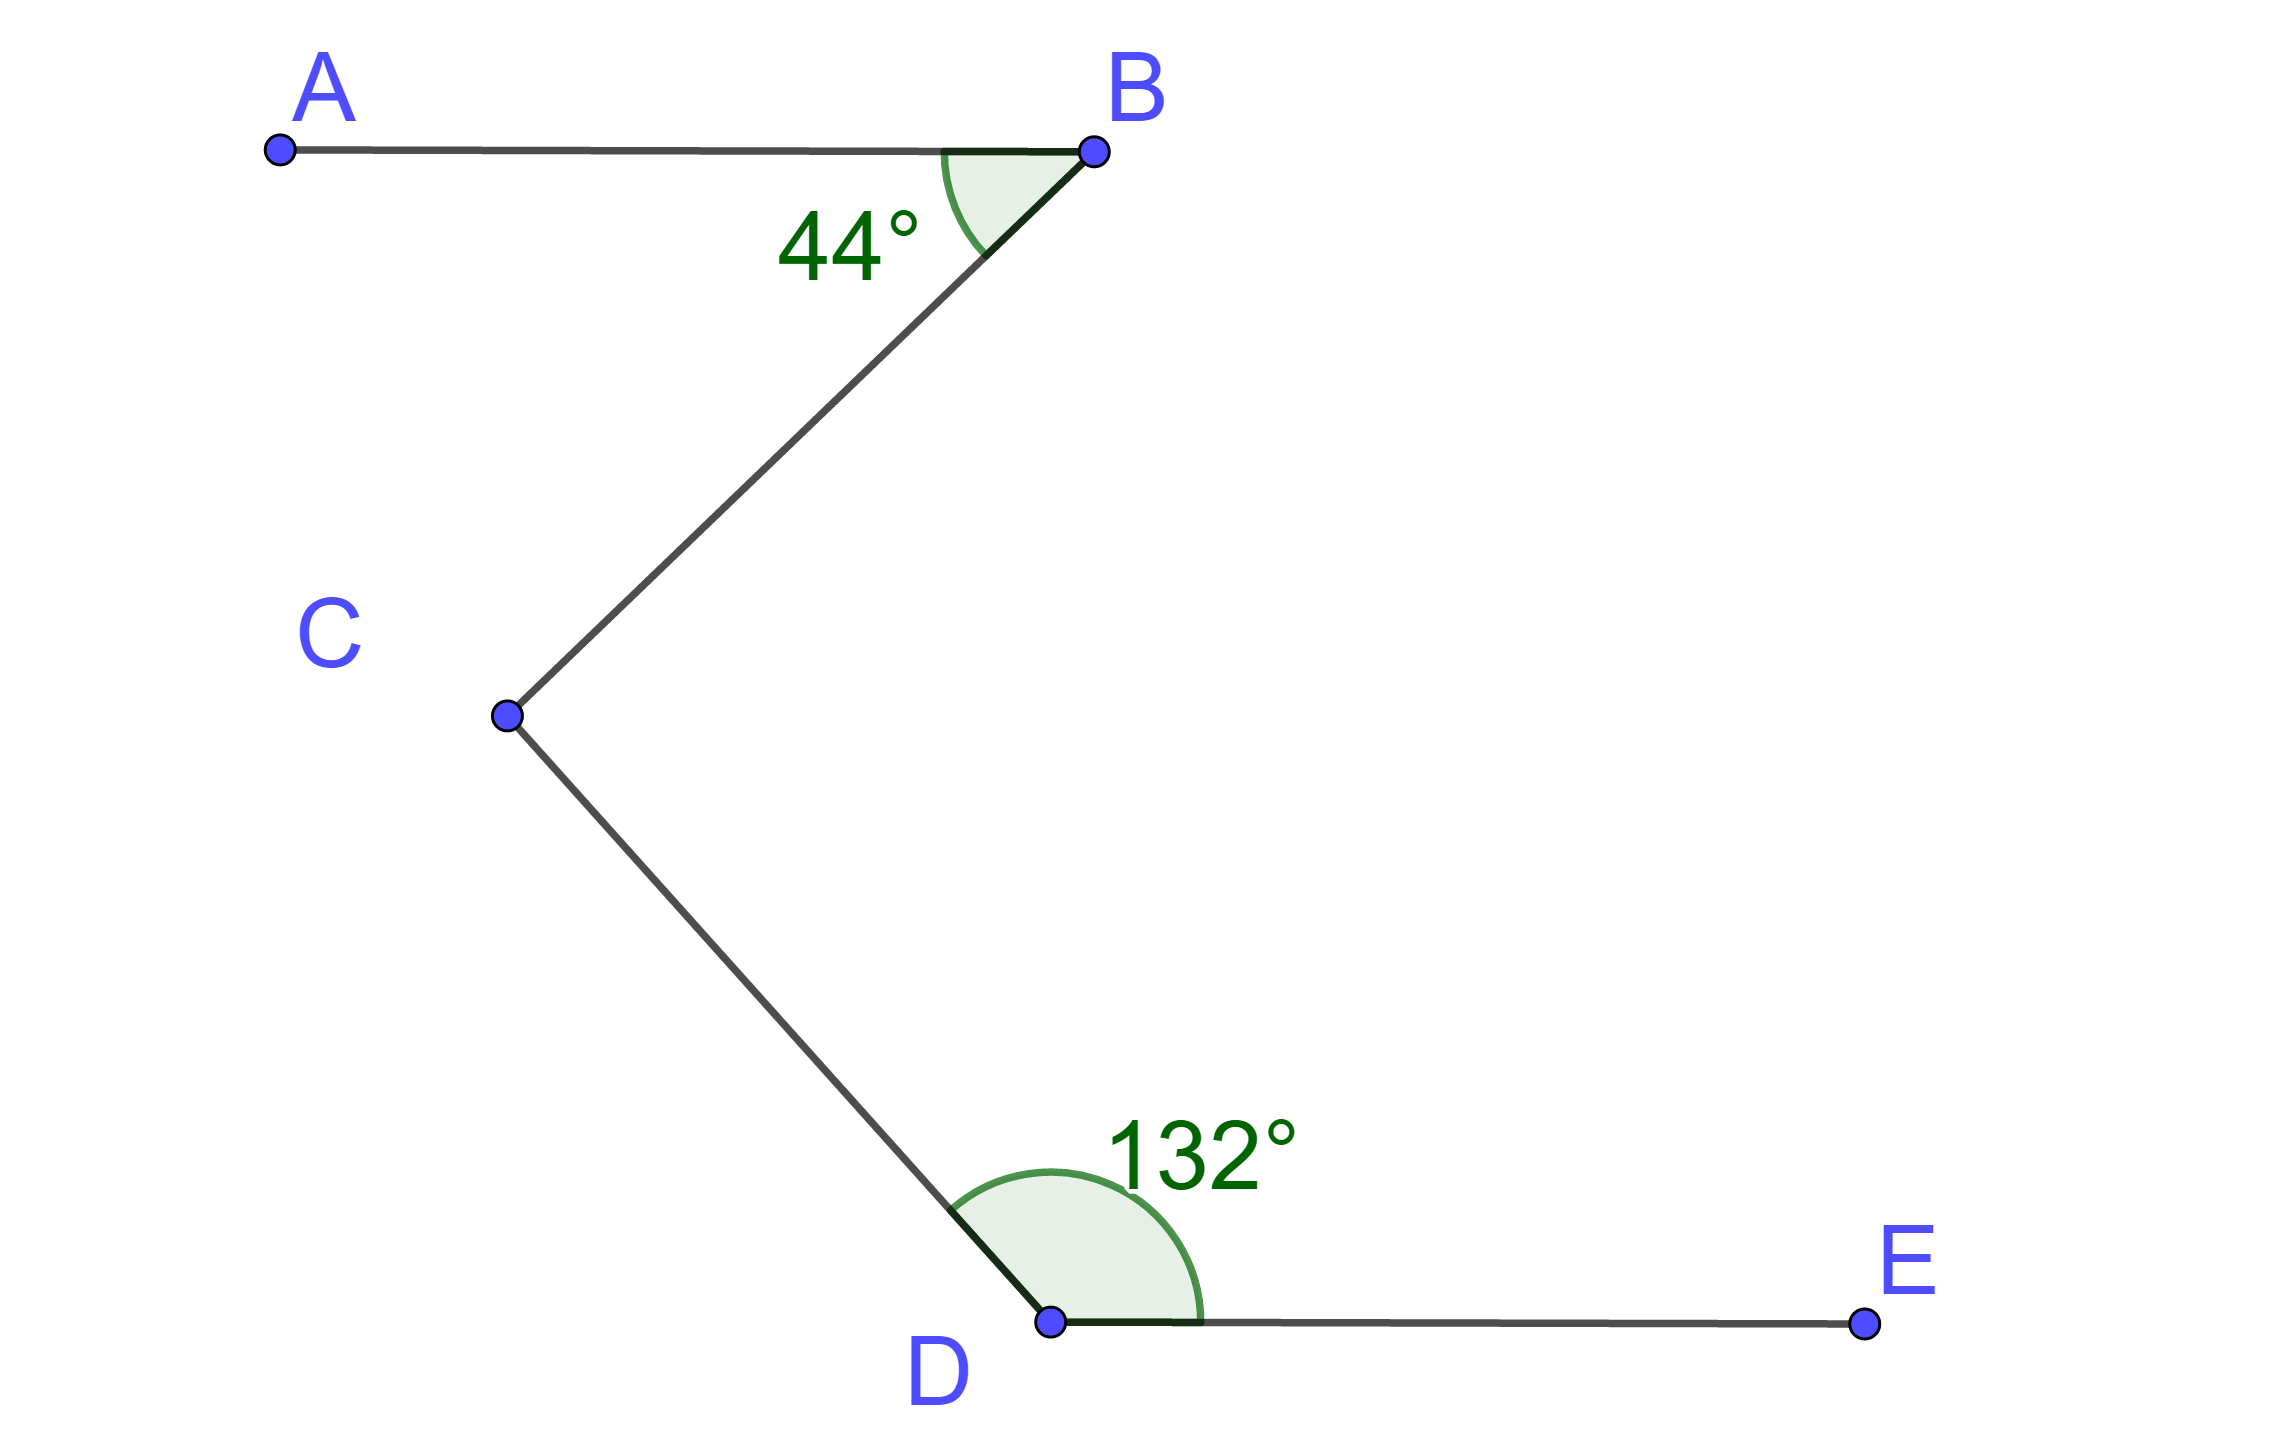
\includegraphics[scale=0.1]{ex37_1}
\end{center}

Je trace la droite parallèle à $(AB)$ et $(DE)$ passant par $C$.

\begin{center}
	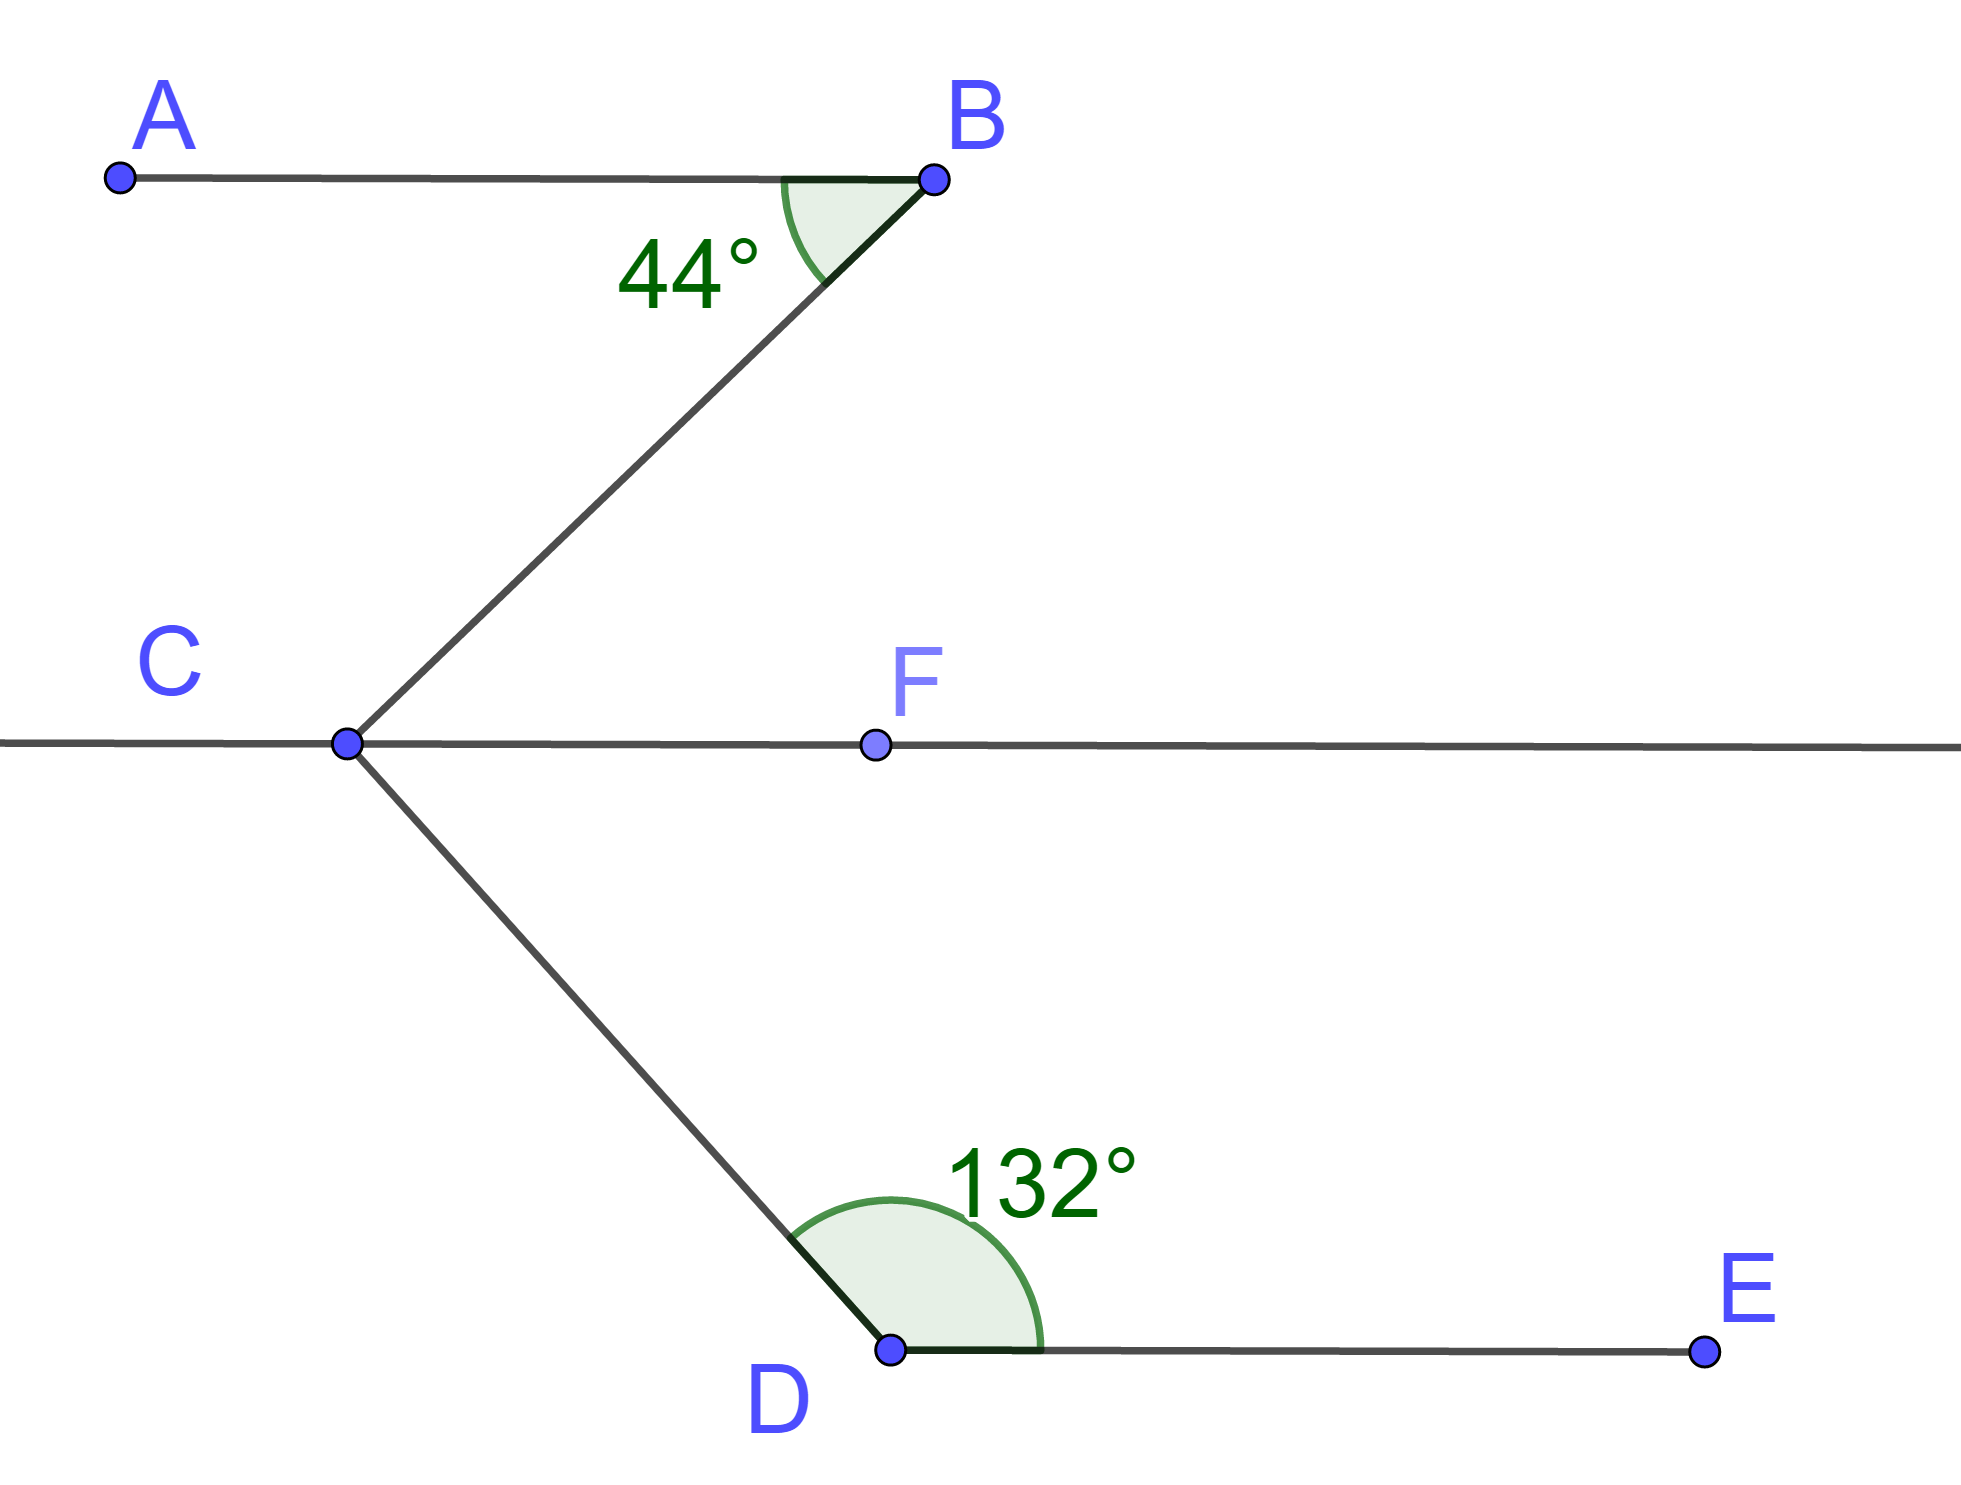
\includegraphics[scale=0.1]{ex37_2}
\end{center}

Les droites $(AB)$ et $(CF)$ sont parallèles et les angles $\widehat{ABC}$ et $\widehat{BCF}$ sont alternes-internes, ils ont la même mesure. Donc $\widehat{BCF}$ = $\widehat{ABC}$ = 44\degree .

\begin{center}
	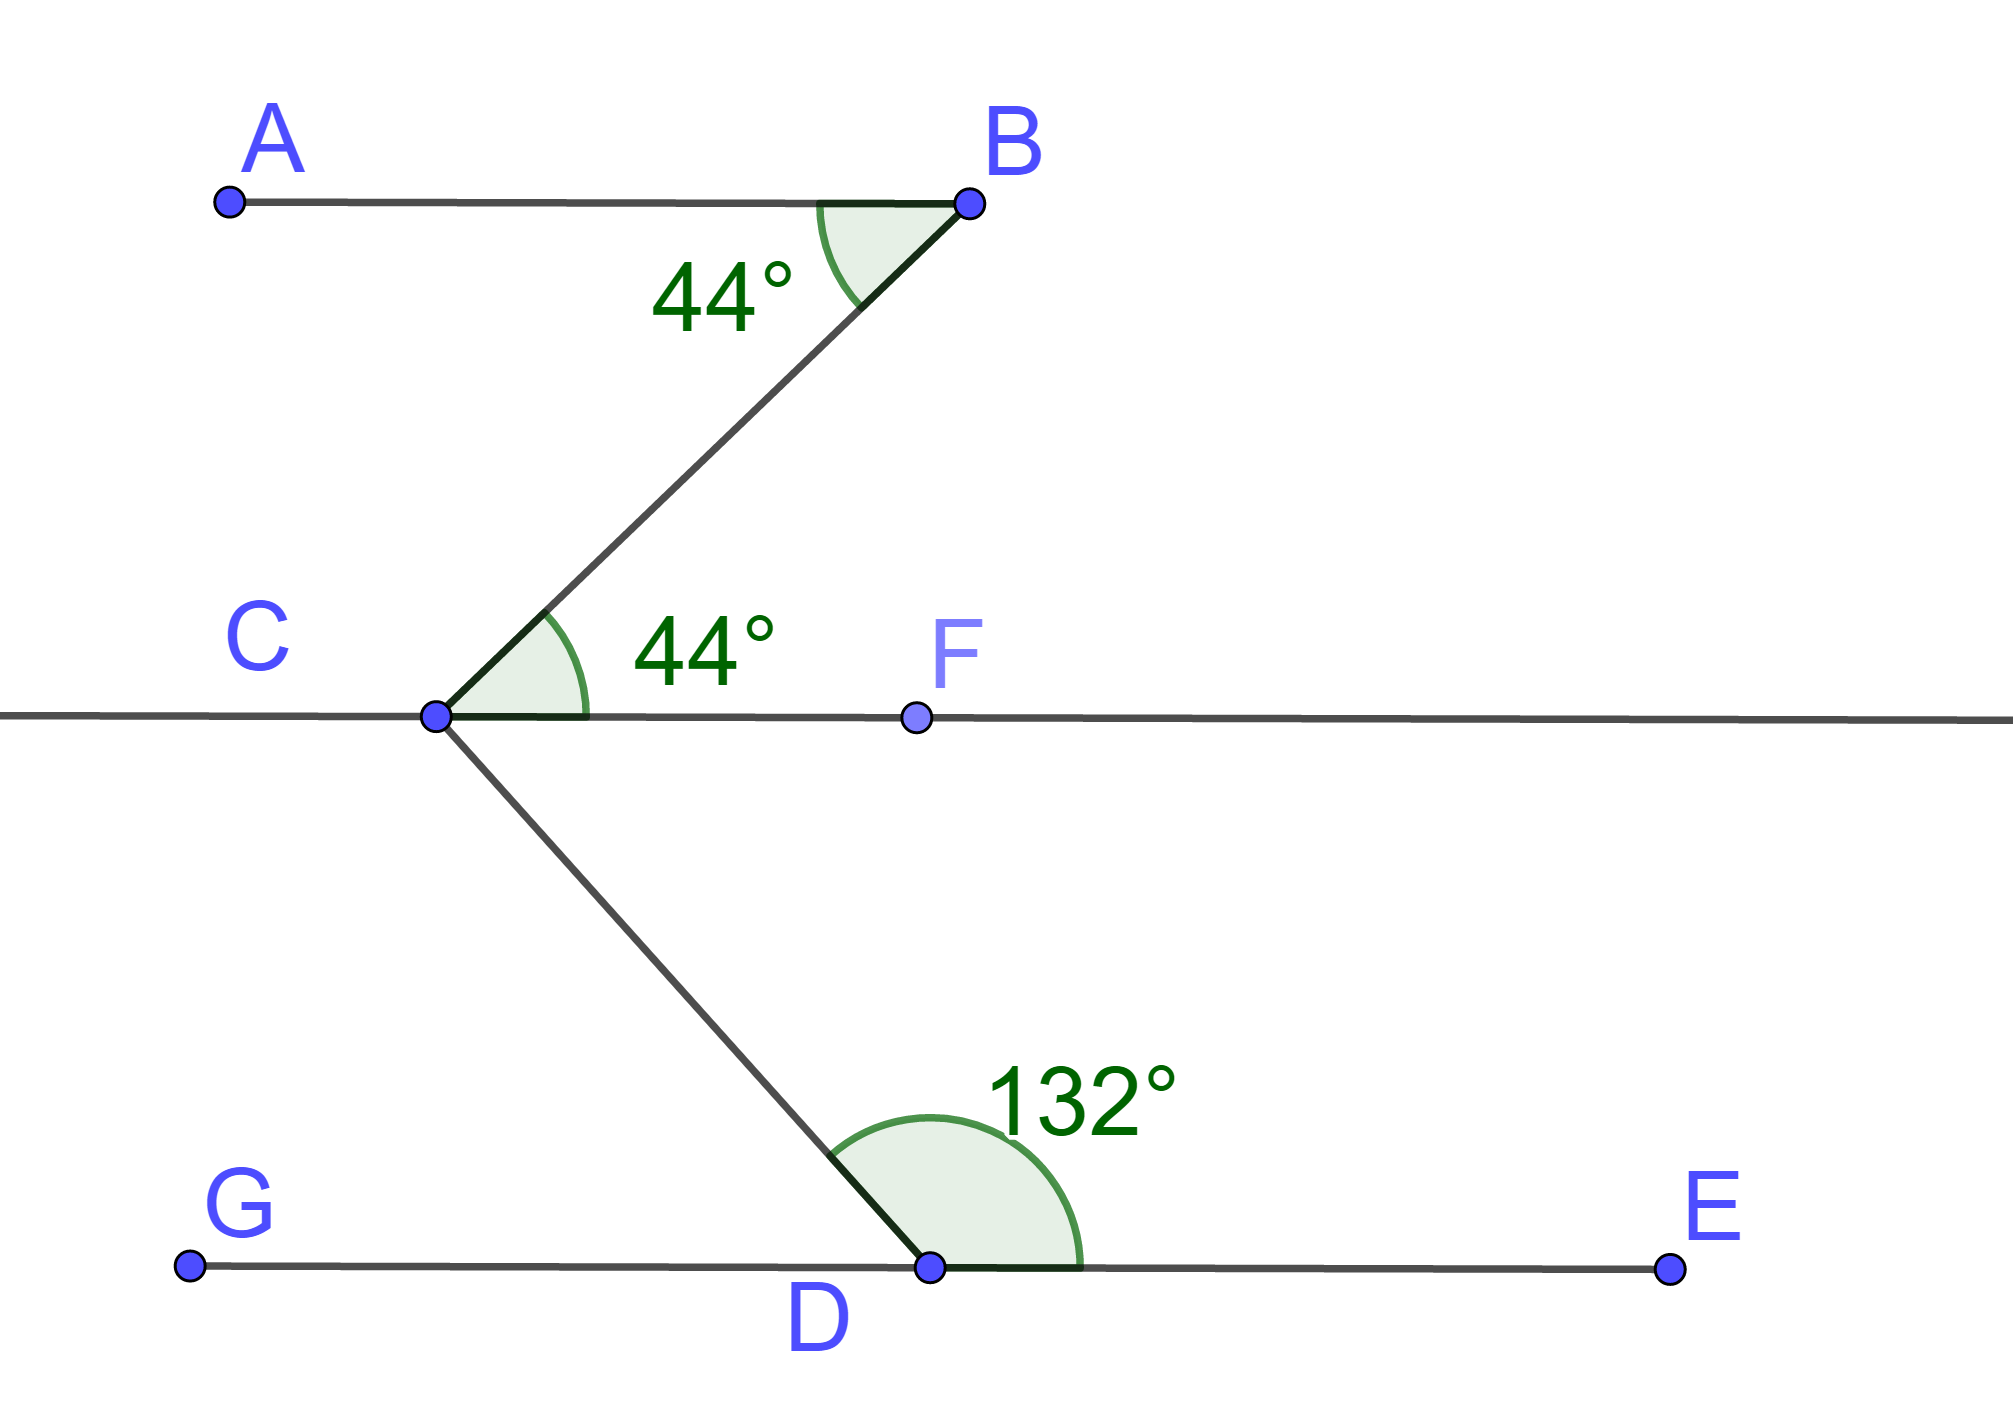
\includegraphics[scale=0.1]{ex37_3}
\end{center}

\newpage

L'angle $\widehat{GDE}$ est plat donc $\widehat{GDC}$ = 180\degree  - 132\degree = 48\degree .
\begin{center}
	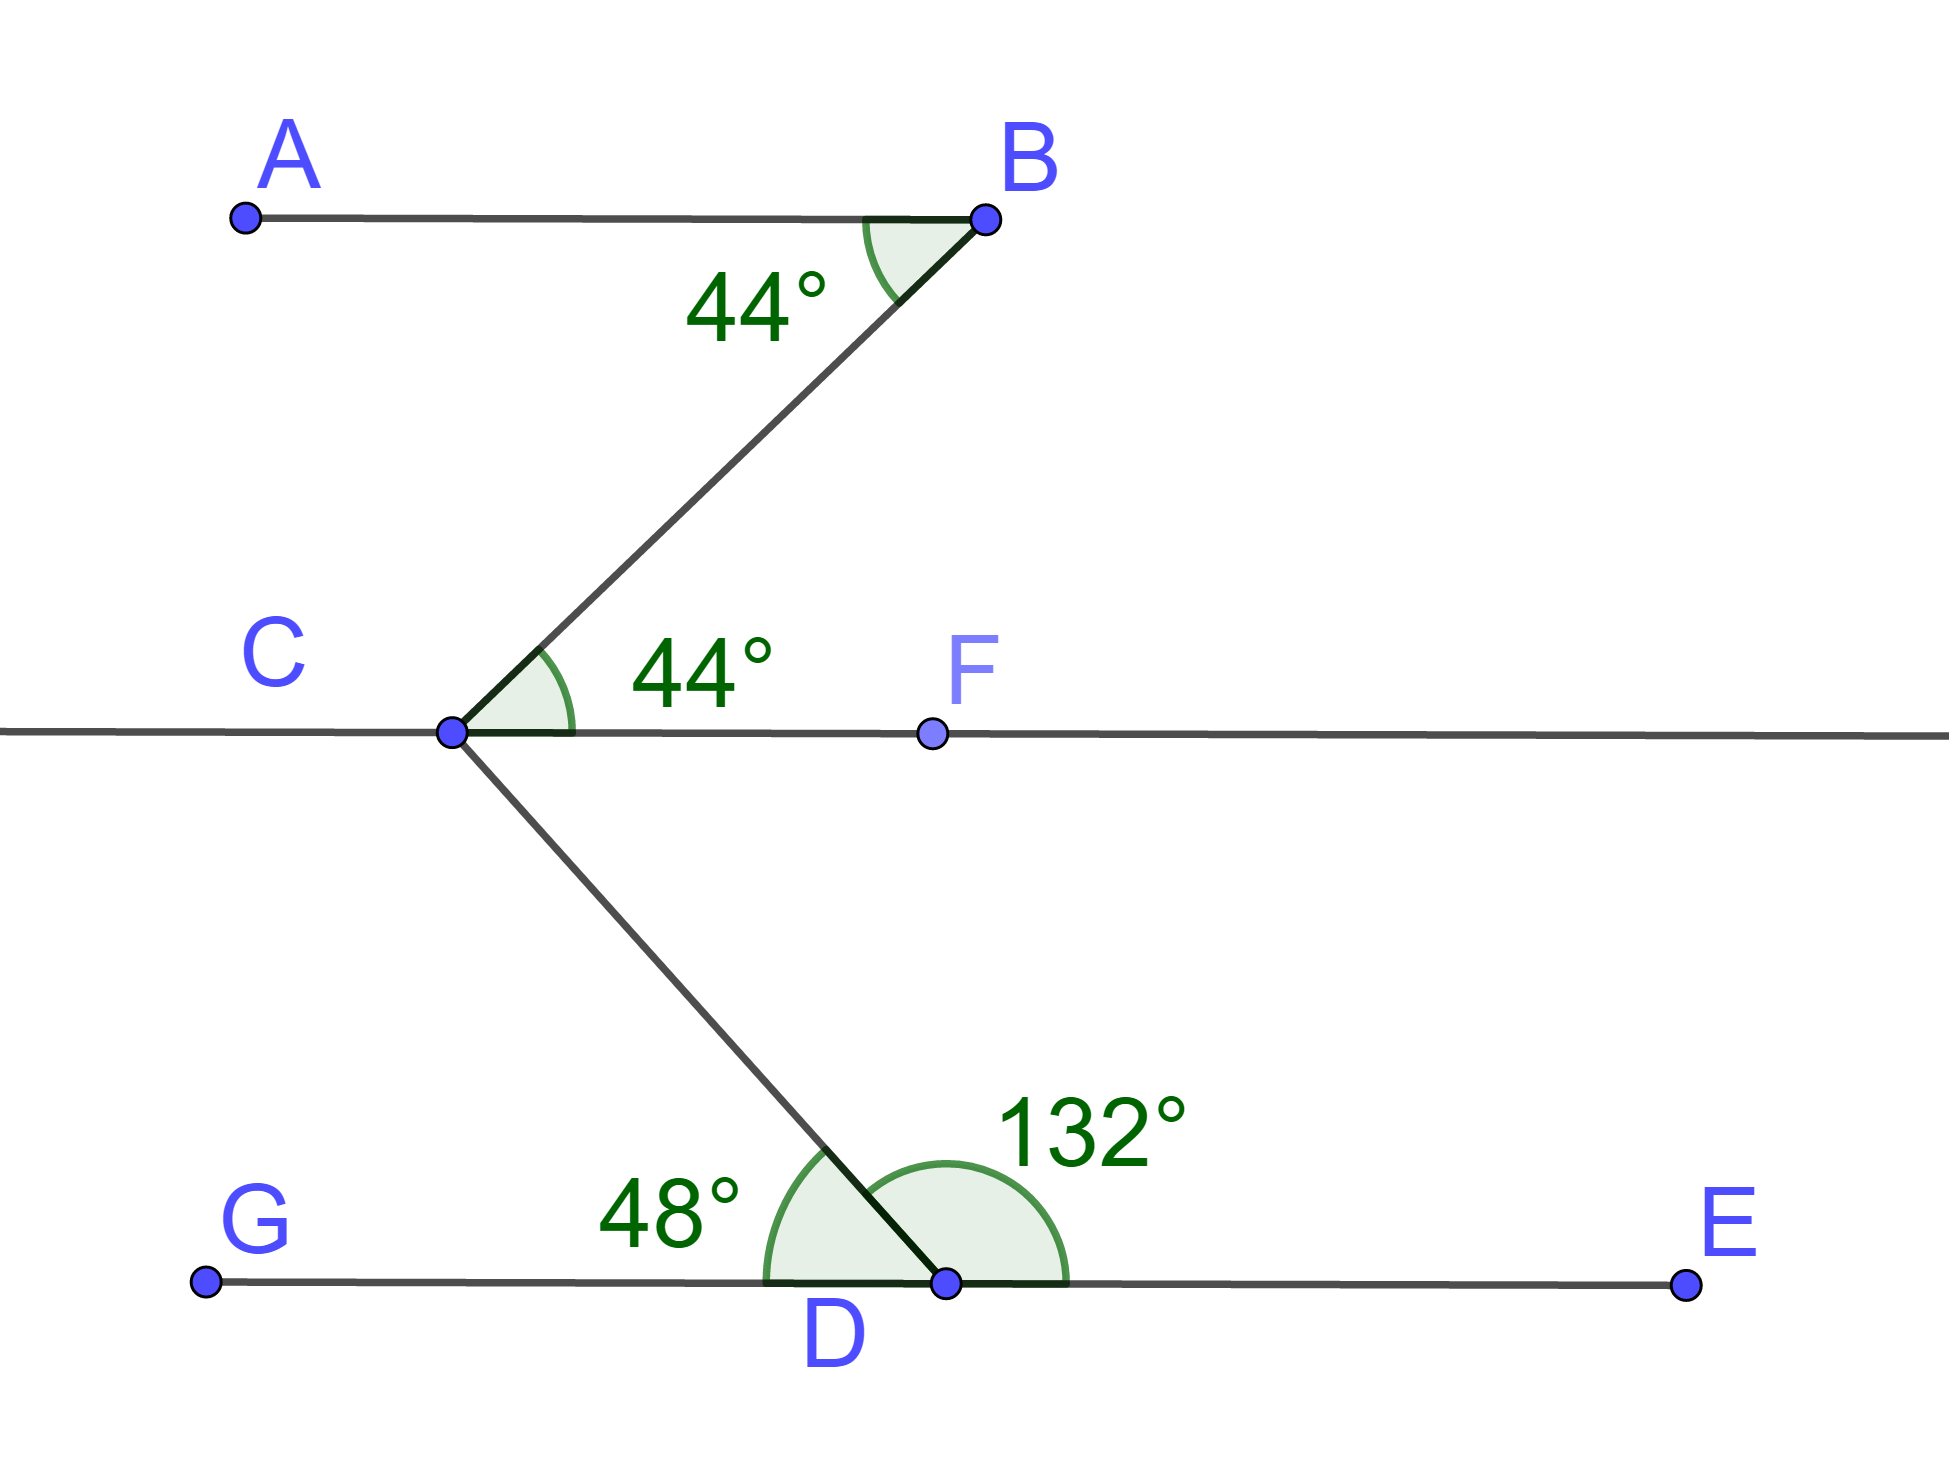
\includegraphics[scale=0.1]{ex37_4}
\end{center}

Les droites $(DE)$ et $(CF)$ sont parallèles et les angles $\widehat{GDC}$ et $\widehat{DCF}$ sont alternes-internes, ils ont la même mesure. Donc $\widehat{DCF}$ = $\widehat{GDC}$ = 48\degree .

\begin{center}
	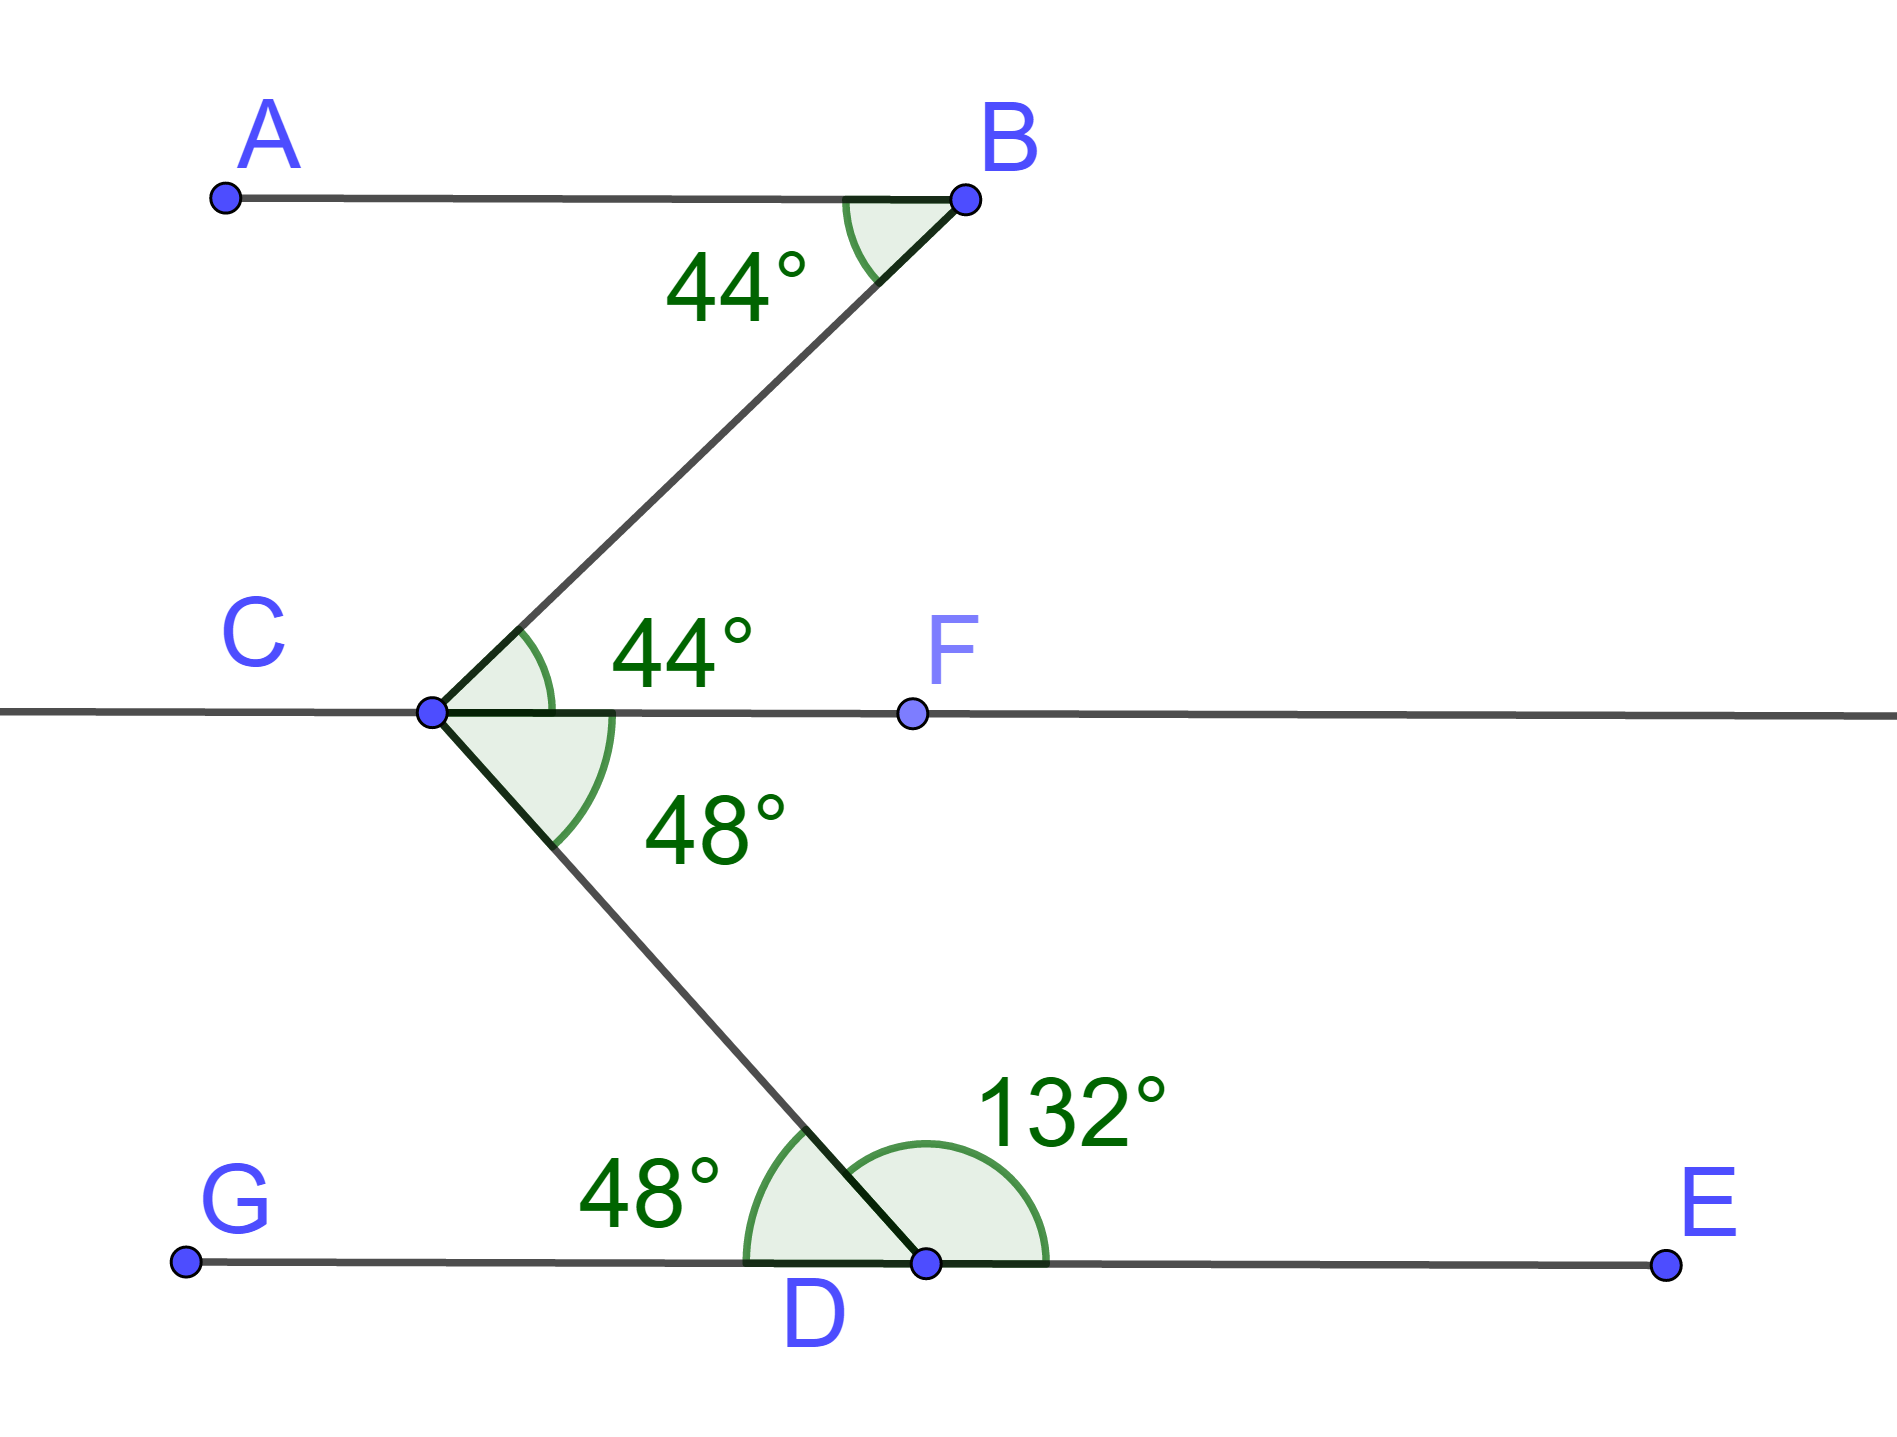
\includegraphics[scale=0.1]{ex37_5}
\end{center}

Donc l'angle $\widehat{BCD}$ mesure 92\degree .


\section*{Exercice 42}

Dans le triangle ABC, la somme des mesure des angles est égale à 180\degree . 

Donc $\widehat{ACB}$ = 180\degree - (52\degree  + 87\degree ) = 41\degree .


Les angles $\widehat{ACB}$ et $\widehat{CED}$ sont correspondants et de même mesure donc les droites $(CB)$ et $(ED)$ sont parallèles.


\section*{Exercice 42}


\begin{enumerate}[label=\alph*.]
	\item \  
	
	\item Dans le triangle BCD, la somme des mesure des angles est égale à 180\degree . 	
	Donc $\widehat{BCD}$ = 180\degree - (45\degree  + 45\degree ) = 90\degree .
	
	Le triangle ABD est équilatéral donc $\widehat{BDA}$ = $\widehat{DAB}$ = $\widehat{ABD}$ = 60\degree .
	
	
	L'angle $\widehat{CDE}$ est plat donc $\widehat{ADE}$ = 180\degree  - (45\degree  + 60\degree ) = 75\degree .
	
	Dans le triangle AED, la somme des mesure des angles est égale à 180\degree . 	
	Donc $\widehat{AED}$ = 180\degree - (75\degree  + 15\degree ) = 90\degree .
	
	\item Je sais que les droites $(AE)$ et $(BC)$ sont perpendiculaires à $(EC)$.
	Or si deux droites sont perpendiculaires à une même troisième alors elles sont parallèles entres elles.
	Donc Les droites $(AE)$ et $(BC)$ sont parallèles.
	
\end{enumerate}


\section*{Exercice 45}

	Dans le triangle KLJ, la somme des mesure des angles est égale à 180\degree . 	
	Donc $\widehat{KLJ}$ = 180\degree - (114\degree  + 38\degree ) = 28\degree .
	
	
	Le triangle ILJ est isocèle en I donc $\widehat{IJL}$ = $\widehat{JLI}$. 
	Dans le triangle ILJ, la somme des mesure des angles est égale à 180\degree . 	
	Donc $\widehat{IJL}$ = (180\degree - 124\degree ) $\div$ 2 = 28\degree .
	
	
	
	Les angles $\widehat{IJL}$ et $\widehat{KLJ}$ sont alternes-internes et de même mesure donc les droites $(LK)$ et $(IJ)$ sont parallèles. Valentin à raison.
\end{document}